\section{Projeto de controladores digitais baseado na resposta em frequência}

\begin{frame}{Resposta em frequência}
\begin{center}
  \scalebox{1}{

\tikzset{every picture/.style={line width=0.75pt}} %set default line width to 0.75pt        

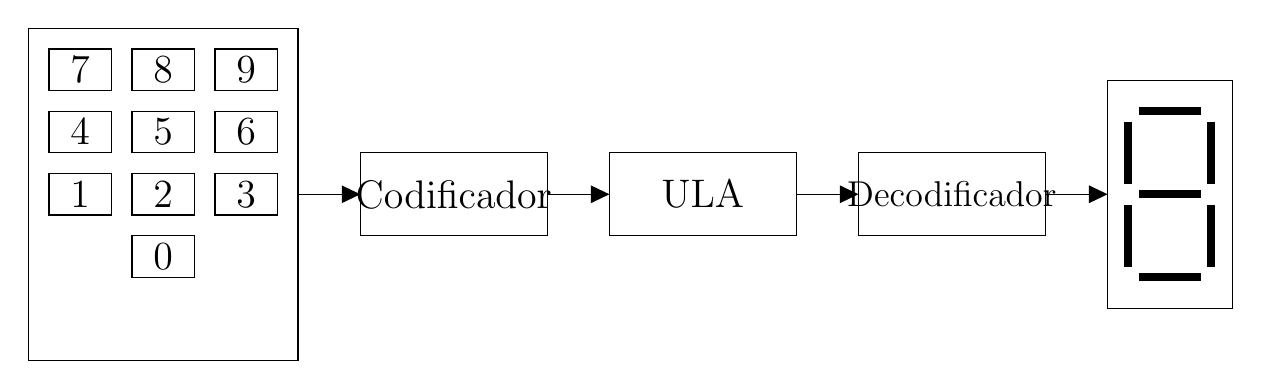
\begin{tikzpicture}[x=0.75pt,y=0.75pt,yscale=-1,xscale=1]
%uncomment if require: \path (0,300); %set diagram left start at 0, and has height of 300

%Shape: Rectangle [id:dp8798188650405219] 
\draw   (30,50) -- (160,50) -- (160,210) -- (30,210) -- cycle ;
%Shape: Rectangle [id:dp593444354888008] 
\draw   (40,60) -- (70,60) -- (70,80) -- (40,80) -- cycle ;
%Shape: Rectangle [id:dp4412846627526852] 
\draw   (80,60) -- (110,60) -- (110,80) -- (80,80) -- cycle ;
%Shape: Rectangle [id:dp2343273962035186] 
\draw   (120,60) -- (150,60) -- (150,80) -- (120,80) -- cycle ;
%Shape: Rectangle [id:dp05777918912875246] 
\draw   (40,90) -- (70,90) -- (70,110) -- (40,110) -- cycle ;
%Shape: Rectangle [id:dp9955010424516375] 
\draw   (80,90) -- (110,90) -- (110,110) -- (80,110) -- cycle ;
%Shape: Rectangle [id:dp24021539717259266] 
\draw   (120,90) -- (150,90) -- (150,110) -- (120,110) -- cycle ;
%Shape: Rectangle [id:dp36169684584711925] 
\draw   (40,120) -- (70,120) -- (70,140) -- (40,140) -- cycle ;
%Shape: Rectangle [id:dp7232437677097003] 
\draw   (80,120) -- (110,120) -- (110,140) -- (80,140) -- cycle ;
%Shape: Rectangle [id:dp6884539525496838] 
\draw   (120,120) -- (150,120) -- (150,140) -- (120,140) -- cycle ;
%Shape: Rectangle [id:dp9961423077173726] 
\draw   (80,150) -- (110,150) -- (110,170) -- (80,170) -- cycle ;
%Shape: Rectangle [id:dp6643057105712631] 
\draw   (190,110) -- (280,110) -- (280,150) -- (190,150) -- cycle ;
%Shape: Rectangle [id:dp7094011053258715] 
\draw   (550,75) -- (610,75) -- (610,185) -- (550,185) -- cycle ;
%Shape: Rectangle [id:dp2693438921699036] 
\draw   (310,110) -- (400,110) -- (400,150) -- (310,150) -- cycle ;
%Shape: Rectangle [id:dp3654960401722005] 
\draw   (430,110) -- (520,110) -- (520,150) -- (430,150) -- cycle ;
%Straight Lines [id:da6667328032348829] 
\draw    (160,130) -- (188,130) ;
\draw [shift={(190,130)}, rotate = 180] [fill={rgb, 255:red, 0; green, 0; blue, 0 }  ][line width=0.75]  [draw opacity=0] (8.93,-4.29) -- (0,0) -- (8.93,4.29) -- cycle    ;

%Straight Lines [id:da5165651690517046] 
\draw    (280,130) -- (308,130) ;
\draw [shift={(310,130)}, rotate = 180] [fill={rgb, 255:red, 0; green, 0; blue, 0 }  ][line width=0.75]  [draw opacity=0] (8.93,-4.29) -- (0,0) -- (8.93,4.29) -- cycle    ;

%Straight Lines [id:da17751850693095572] 
\draw    (400,130) -- (428,130) ;
\draw [shift={(430,130)}, rotate = 180] [fill={rgb, 255:red, 0; green, 0; blue, 0 }  ][line width=0.75]  [draw opacity=0] (8.93,-4.29) -- (0,0) -- (8.93,4.29) -- cycle    ;

%Straight Lines [id:da4998570413390182] 
\draw [color={rgb, 255:red, 0; green, 0; blue, 0 }  ,draw opacity=1 ][line width=3]    (560,95) -- (560,125) ;


%Straight Lines [id:da05287212083080073] 
\draw [color={rgb, 255:red, 0; green, 0; blue, 0 }  ,draw opacity=1 ][line width=3]    (600,95) -- (600,125) ;


%Straight Lines [id:da9146969001147236] 
\draw [color={rgb, 255:red, 0; green, 0; blue, 0 }  ,draw opacity=1 ][line width=3]    (560,135) -- (560,165) ;


%Straight Lines [id:da37610179690179124] 
\draw [color={rgb, 255:red, 0; green, 0; blue, 0 }  ,draw opacity=1 ][line width=3]    (600,135) -- (600,165) ;


%Straight Lines [id:da2798262228013664] 
\draw [color={rgb, 255:red, 0; green, 0; blue, 0 }  ,draw opacity=1 ][line width=3]    (595,130) -- (565,130) ;


%Straight Lines [id:da15184615547446478] 
\draw [color={rgb, 255:red, 0; green, 0; blue, 0 }  ,draw opacity=1 ][line width=3]    (595,90) -- (565,90) ;


%Straight Lines [id:da20609816632014244] 
\draw [color={rgb, 255:red, 0; green, 0; blue, 0 }  ,draw opacity=1 ][line width=3]    (595,170) -- (565,170) ;


%Straight Lines [id:da16937059284664002] 
\draw    (520,130) -- (548,130) ;
\draw [shift={(550,130)}, rotate = 180] [fill={rgb, 255:red, 0; green, 0; blue, 0 }  ][line width=0.75]  [draw opacity=0] (8.93,-4.29) -- (0,0) -- (8.93,4.29) -- cycle    ;


% Text Node
\draw (135,70) node   {\Large $9$};
% Text Node
\draw (95,70) node   {\Large $8$};
% Text Node
\draw (55,70) node   {\Large $7$};
% Text Node
\draw (135,100) node   {\Large $6$};
% Text Node
\draw (135,130) node   {\Large $3$};
% Text Node
\draw (95,160) node   {\Large $0$};
% Text Node
\draw (95,130) node   {\Large $2$};
% Text Node
\draw (95,100) node   {\Large $5$};
% Text Node
\draw (55,100) node   {\Large $4$};
% Text Node
\draw (55,130) node   {\Large $1$};
% Text Node
\draw (235,130) node  [align=left] {\Large Codificador};
% Text Node
\draw (355,130) node  [align=left] {\Large ULA};
% Text Node
\draw (475,130) node [scale=0.9] [align=left] {\Large Decodificador};


\end{tikzpicture}
}  
\end{center}
\begin{block}{Considerando o sistema acima:}
$ x(t) = $ entrada;\\
$ h(t) = $ resposta ao impulso;\\
$ y(t) = $ saída.\\
\vspace{0.3 cm}
\begin{minipage}[t]{0.48\linewidth}
    \centering
        \textbf{Caso contínuo:}\\
	    $y(t) = h(t) \circledast x(t)$ \\
	    $Y(j\omega) = \bm{H(j\omega)}\cdot X(j\omega)$
\end{minipage}\hfill
\begin{minipage}[t]{0.48\linewidth}
    \centering
        \textbf{Caso discreto:}\\
	    $y[n] = h[n] \circledast x[n]$ \\
	    $Y(e^{j\omega}) = \bm{H(e^{j\omega})}\cdot X(e^{j\omega})$
\end{minipage}

\vspace{0.3 cm}
\textbf{Definição:} A \textbf{resposta em frequência} de um sistema é definida como a transformada de Fourier da resposta ao impulso!
\end{block}
\end{frame}

\begin{frame}{Interpretação física}
\begin{block}{Entrada senoidal}
	\begin{equation*}
	    x(t) = A \cdot sen(\omega_{0}t)
	\end{equation*}
onde $A$ é a  amplitude, $ \omega_{0} $ é a frequência em rad/s e a fase, neste caso, é $\SI{0}{\degree}$.
\vspace{0.3 cm}
\begin{itemize}
    \item Em estado \textbf{estacionário} $y(t)$ também será uma oscilação pura.
    \item $ \omega_{0} $ não muda;
    \item A amplitude e a fase podem mudar, mas como?
    \item Quem responde se esses parâmetros aumentam ou diminuem é a \textbf{resposta em frequência}!
\end{itemize}
\end{block}
\end{frame}

\begin{frame}{Interpretação física}
\begin{block}{Em termos matemáticos:}
\begin{itemize}
    \item Que operação matemática única pode alterar amplitude e fase simultaneamente e de forma independente?\\
    \vspace{0.3 cm}
    \textbf{Um produto por um número complexo!}
    \vspace{0.3 cm}
        \item Analisando cada frequência da entrada de maneira individual, cada função complexa vira um número complexo distinto.
\end{itemize}
\vspace{0.2 cm}
    $$\boxed{ y(t)= |H(j\omega_{0})| \ \text{sen}\left(\omega_{0}t + \phase{H(j\omega_{0})}\right)}$$
\end{block}
\end{frame}

\begin{frame}{Interpretação física - Exemplo \#01}
    \begin{block}{Problema}
        Considere a equação diferencial:\\
        \begin{center}
            $\dot{y}(t) + ay(t) = x(t)$, $ a > 0 $ \\
            \vspace{0.3cm}
            $ H(j\omega) = \dfrac{1}{j\omega + a} $\\
            \vspace{0.3cm}
            $ h(t) = \text{e}^{-at}u(t)$, $ a > 0 $\\
        \end{center}
        \begin{itemize}
            \item Supondo $ \omega = \omega_{0} $:
        \end{itemize}
    \begin{equation*}
        H(j\omega_{0}) =  \dfrac{1}{j\omega_{0} + a}
    \end{equation*}
\end{block}
\end{frame}

\begin{frame}{Interpretação física - Exemplo \#01}
\centerline{\includegraphics[width=0.8\linewidth]{Figuras/Ch13/fig1.png}}
\end{frame}

\begin{frame}{Interpretação física - Exemplo \#01}
    \begin{block}{Resolução}
    \begin{itemize}
        \item É possível determinar ganho e fase diretamente pelo gráfico:
    \end{itemize}
        \begin{center}
            $ K = \dfrac{A}{B} = \num{0,3162} $\\
            \vspace{0.2cm}
            $ \phi = -\num{1,26}$ rad\\
        \end{center}
    \vspace{0.3 cm}
    \begin{itemize}
        \item Ou tirar a informação diretamente da resposta em frequência:
    \end{itemize}
        \begin{equation*}
            K = \left| \dfrac{1}{j3 + 1}\right|
            \qquad \phi = \phase{\scriptstyle \dfrac{1}{j3 + 1}}
        \end{equation*}
\end{block}
\end{frame}

\begin{frame}{Interpretação física - Exemplo \#01}
\centerline{\includegraphics[width=0.8\linewidth]{Figuras/Ch13/fig2.png}}
\end{frame}

\begin{frame}{Interpretação física - Exemplo \#02}
\begin{block}{Problema}
\vspace{0.2cm}
    \begin{equation*}
        y[n] - \frac{3}{4} y[n-1] + \frac{1}{8} y[n - 2] = 2 x[n]
    \end{equation*}
    Aplicando a transformada de Fourier, temos:\\
    \begin{equation*}
        H(\text{e}^{j\omega}) = \dfrac{Y(\text{e}^{j\omega})}{X(\text{e}^{j\omega})} = \dfrac{2}{1 - \dfrac{3}{4} \text{e}^{-j\omega} + \dfrac{1}{8} \text{e}^{-2 j\omega}}
    \end{equation*}
\end{block}
\end{frame}

\begin{frame}{Interpretação física - Exemplo \#02}
\centerline{\includegraphics[width=0.7\linewidth]{Figuras/Ch13/fig3.png}}
\vspace{-0.35cm}
	\begin{block}{Para $ \omega_{0} = \pi/10 $ rad/s:}
\begin{minipage}[t]{0.48\linewidth}
    \centering
        \textbf{Gráfico:}\\
	    $ K = \num{4,7617} $ \\
	    $ \phi = -\num{0,3142} $ rad \\
\end{minipage}\hfill
\begin{minipage}[t]{0.48\linewidth}
    \centering
        \textbf{Função:}\\
	    $ K = \num{4,7737} $ \\
	    $ \phi = -\num{0,3875} $ rad \\
\end{minipage}
\end{block}
\end{frame}

\begin{frame}{Representação gráfica da resposta em frequência}
    \begin{block}{Diagrama de Bode}
    \begin{itemize}
        \item Hendrik Wade Bode mostrou que, tanto o logaritmo do módulo como a fase da  resposta em frequência de sistemas contínuos  podem ser aproximados por retas, chamadas  assíntotas, ao usar uma escala logarítmica  para a frequência.
        \item Devido a presença de funções \textbf{transcedentais}, nos diagramas de Bode \textbf{discretos} as relações  entre o logaritmo do módulo e da fase com  a frequência não mais podem ser aproximados por retas assíntotas.
        \item Podem ser obtidos por meio de recursos computacionais, calculando-se os pontos numericamente através da relação $ z = \text{e}^{sT} $.
    \end{itemize}
    \end{block}
\end{frame}

\begin{frame}{Representação gráfica da resposta em frequência - Exemplo \#01}
\begin{block}{Problema}
\vspace{0.2cm}
    \begin{equation*}
        G(s) = \dfrac{1}{s(s + 1)}
    \end{equation*}
\end{block}
\end{frame}

\begin{frame}{Representação gráfica da resposta em frequência - Exemplo \#01}
\begin{block}{Resolução}
\begin{itemize}
    \item Discretizando por ZOH:
\end{itemize}
    \begin{equation*}
        G_1(z) = \dfrac{0.01873z + 0.01752}{z^2 - 1.819z + 0.8187} \text{  p/  } T = 0.2 s
    \end{equation*}
    \begin{equation*}
        G_2(z) = \dfrac{0.3679z + 0.2642}{z^2 - 1.368z + 0.3679} \text{  p/  } T = 1 s
    \end{equation*}
    \begin{equation*}
        G_3(z) = \dfrac{1.135z + 0.594}{z^2 - 1.135z + 0.1353} \text{  p/  } T = 2 s
    \end{equation*}
\end{block}
\end{frame}

\begin{frame}{Representação gráfica da resposta em frequência - Exemplo \#01}
\centerline{\includegraphics[width=0.9\linewidth]{Figuras/Ch13/fig4.png}}
\end{frame}

\begin{frame}{Formas de mapeamento}
    \begin{block}{Transformação bilinear}
    Para desenhar assíntotas seria necessário voltar a ter uma relação linear na frequência. Isso pode ser obido utilizando a relação bilinear (\textit{evitando a utilização de funções transcendentais}). \\
    \vspace{0.3 cm}
    \textbf{Arnold Tustin:} \textit{A method of analysing the behaviour of linear systems in terms of time series (1947)}\\
    \vspace{0.3 cm}
    \begin{equation*}
        \text{ln}(z) \approx 2 \left(\dfrac{z - 1}{z + 1}\right) \implies w = \dfrac{2}{T}\left(\dfrac{z - 1}{z + 1}\right)
    \end{equation*}
    \end{block}
\end{frame}

\begin{frame}{Mapeamento entre os planos $s$, $z$ e $w$}
\centerline{\includegraphics[width=1\linewidth]{Figuras/Ch13/fig5.png}}
	\begin{block}{}
	A principal diferença entre os planos $s$ e $w$ é que enquanto no plano $s$ a frequência $\omega$ está na faixa de $ -\pi/T \leq \omega \leq +\pi/T$, no plano $w$ a frequência $\omega_w $ está na faixa de $ -\infty < \omega_w < +\infty $.
	\end{block}
\end{frame}

\begin{frame}{Mapeamento entre os planos $s$, $z$ e $w$}
    \begin{block}{Relação entre $\omega$ e $\omega_w$}
	$$ w = j\omega_w \implies \omega_w = \frac{2}{T} \text{tan} \frac{\omega T}{2} $$
	\vspace{-0.3cm}
	\begin{itemize}
	    \item Para $\omega T$ pequenos temos, $\omega_w \approx \omega$. 
	    \item Na prática, a aproximação é aceitável se $ \omega \leq \omega_s/10$!
	\end{itemize}
	\end{block}
\centerline{\includegraphics[width=0.5\linewidth]{Figuras/Ch13/fig6.png}}
\end{frame}

\begin{frame}{Mapeamento entre os planos $s$, $z$ e $w$ - Exemplo \#01}
\scalebox{0.6}{\deftkzbds
	
\begin{tikzpicture}[auto, node distance=2cm,>=Latex]
	
	\node [input, name=input] {};
	
	\node [coordinate, right=of input] (junction) {};
	\draw (input) -- node[near start] {$E(z)$} (junction);
	
	\node [block, right=of junction] (ei) {$ C_i(z) $};
	\node [block, above=of ei] (kp) {$ C_p(z) $};
	\node [block, below=of ei] (cd) {$ C_d(z) $};
	
	\draw [->] (junction) -- (ei);
	\draw [->] (junction) |- (kp);
	\draw [->] (junction) |- (cd);
	
	\node [sum, right=2cm of ei] (sum) {$ \phantom{\sum} $};
	\draw (sum) ++(-8pt,-8pt) -- ++(16pt,16pt) ++(-16pt,0pt) -- +(16pt,-16pt);
	
	\draw [<-] (sum) -- node[very near start, above] {$ + $} (ei);
	\draw [<-] (sum) |- node[very near start, right] {$ + $} (kp);
	\draw [<-] (sum) |- node[very near start, left] {$ + $} (cd);
	
	\node [output, right=of sum] (output) {};
	\draw [->] (sum) -- node[near end] {$ U(z) $} (output);
\end{tikzpicture}}
	\begin{block}{Subsistema D/A + processo + A/D}
\vspace{0.2cm}
	\begin{equation*}
	    G_p(z) = \dfrac{Y(z)}{U(z)} = (1 - z^{-1})\mathcal{Z}\left[\dfrac{G_p(s)}{s}\right] = (1 - z^{-1})\mathcal{Z}\left[\dfrac{1}{s^2(s + 1)}\right]
	\end{equation*}
	\begin{equation*}
	    G_p(z) = \dfrac{\num{0,0187}(z + \num{0,9355})}{z^2 - \num{1,8187}z + \num{0,8187}} \text{ com  } T = \num{0,2} \text{\ s}
	\end{equation*}
	\end{block}
\end{frame}

\begin{frame}{Mapeamento entre os planos $s$, $z$ e $w$ - Exemplo \#01}
	\begin{block}{Usando a transformação bilinear com $T = \num{0,2}$ s}
	\centering
	   $ z = \dfrac{2 + Tw}{2 - Tw} = \dfrac{2 + \num{0,2}w}{2 - \num{0,2}w} = \dfrac{1 + \num{0,1}w}{1 - \num{0,1}w} $
	\begin{align*}
		G_p(w)&=\dfrac{\num{0,0187}\left[\left(\frac{1 + \num{0,1}w}{1 - \num{0,1}w}\right) + \num{0,9355})\right]}{\left(\frac{1 + \num{0,1}w}{1 - \num{0,1}w}\right)^2 - \num{1,8187}\left(\frac{1 + \num{0,1}w}{1 - \num{0,1}w}\right) + \num{0,8187}}\\
		&=\dfrac{\num{0,0187}[-\num{0,000645}w^2 - \num{0,1871}w + \num{1,9355}]}{\num{0,036374}w^2 + \num{0,03626}w} \\
		&\approx \dfrac{\num{0,000333}[-w^2 -290w + 3000]}{w^2 + w} \\
		&\approx \dfrac{\num{0,000333}(w + 300)(-w + 10)}{w(w + 1)} \approx \dfrac{\left(\frac{w}{300} + 1\right) \left(-\frac{w}{10} + 1\right)}{w(w + 1)}
		\end{align*}
	\end{block}
\end{frame}

\begin{frame}{Mapeamento entre os planos $s$, $z$ e $w$ - Exemplo \#01}
	\begin{block}{Considerações $G_p(s)$ \textit{versus} $G_p(w)$ }
	\begin{itemize}
	    \item Os polos de $G_p(j\omega)$ são iguais aos de $G_p(j\omega_w)$. Porém $G_p(w)$ é um sistema de fase não mínima. 
        \item Podemos obter os diagramas de módulo através da soma das assíntotas dos termos fatorados, utilizando a unidade dB. 
        \item Os diagramas de fase podem ser obtidos através da soma de cada um dos termos fatorados. 
	\end{itemize}
	\end{block}
\end{frame}

\begin{frame}{Mapeamento entre os planos $s$, $z$ e $w$ - Exemplo \#01}
\centerline{\includegraphics[width=0.85\linewidth]{Figuras/Ch13/fig8.png}}
\end{frame}

\begin{frame}{Mapeamento entre os planos $s$, $z$ e $w$ - Exemplo \#01}
\begin{block}{Considerações $G_p(s)$ \textit{versus} $G_p(w)$ }
	\begin{itemize}
	    \item Em baixas frequências os gráficos são semelhantes.
        \item Na alta frequência, entretanto
    \end{itemize}
$$ \lim_{w \to \infty} \left | G_p(j\omega) \right | = 0 \to -\infty \text{ dB}$$
    \begin{itemize}
        \item[] enquanto
    \end{itemize}
$$\lim_{\omega_w \to \infty} \left | G_p(j\omega_w) \right | = \lim_{\omega_w \to \infty} \left | \dfrac{\left ( \frac{j\omega_w}{300} + 1\right ) \left ( -\frac{j\omega_w}{10} +1 \right )}{j\omega_w(j\omega_w+1)} \right |= \dfrac{1}{3000}\approx - 69,5 \text{ dB}$$
    \begin{itemize}
        \item A explicação para isso está na região de interesse: $ 0 \leq \omega \leq \pi/T $.
        \item O zero de fase não mínima gera uma distorção na fase de $G_p(j\omega_w)$.
        \item Porém nas baixas e altas frequências as fases são equivalentes.
    \end{itemize}
$$\lim_{\omega \to \infty} \phase{G_p(j\omega)}  = \lim_{\omega_w \to \infty} \phase{G_p(j\omega_w)} = -\ang{180}$$
\end{block}
\end{frame}

\begin{frame}{Projeto do controlador}
    \begin{block}{Considerações iniciais}
    O projeto baseado na resposta em frequência é indicado quando as especificações são dadas em termos dos \textbf{erros estacionários e das margens de ganho e fase}. Em relação a essas especificações podemos definir qual dos compensadores vistos pode ser utilizado.
    \begin{itemize}
        \item A compensação por \textbf{avanço de fase} melhora as margens de estabilidade e aumenta a banda passante, fazendo com que a resposta transitória se torne mais rápida. A desvantagem é o possível aumento de ruídos.
        \item A compensação por \textbf{atraso de fase} melhora a margem de fase com a redução do ganho em altas frequências, deixando a resposta transitória mais lenta. Pode ser utilizado para manter a margem de fase e aumentar o ganho em baixa frequência, reduzindo assim o erro estacionário.
        \item O controlador \textbf{PID} é um tipo de compensador por \textbf{avanço (PD)} e \textbf{atraso (PI)}.
    \end{itemize}
    \end{block}
\end{frame}

\begin{frame}{Projeto do controlador - Exemplo \#01}
    \begin{block}{Problema}
    Deseja-se projetar um controlador $G_c(z)$ de modo a satisfazer às seguintes especificações:
    \begin{itemize}
        \item erro estacionário $e(\infty) = \num{0,3}$ para entrada de referência do tipo rampa unitária;
        \item margem de fase PM $\approx \ang{50}$.
    \end{itemize}
    \end{block}
\centering
\vspace{0.5cm}
\scalebox{0.6}{\deftkzbds
	
\begin{tikzpicture}[auto, node distance=2cm,>=Latex]
	
	\node [input, name=input] {};
	
	\node [coordinate, right=of input] (junction) {};
	\draw (input) -- node[near start] {$E(z)$} (junction);
	
	\node [block, right=of junction] (ei) {$ C_i(z) $};
	\node [block, above=of ei] (kp) {$ C_p(z) $};
	\node [block, below=of ei] (cd) {$ C_d(z) $};
	
	\draw [->] (junction) -- (ei);
	\draw [->] (junction) |- (kp);
	\draw [->] (junction) |- (cd);
	
	\node [sum, right=2cm of ei] (sum) {$ \phantom{\sum} $};
	\draw (sum) ++(-8pt,-8pt) -- ++(16pt,16pt) ++(-16pt,0pt) -- +(16pt,-16pt);
	
	\draw [<-] (sum) -- node[very near start, above] {$ + $} (ei);
	\draw [<-] (sum) |- node[very near start, right] {$ + $} (kp);
	\draw [<-] (sum) |- node[very near start, left] {$ + $} (cd);
	
	\node [output, right=of sum] (output) {};
	\draw [->] (sum) -- node[near end] {$ U(z) $} (output);
\end{tikzpicture}}
\end{frame}

\begin{frame}{Projeto do controlador - Exemplo \#01}
    \begin{block}{Resolução}
\begin{itemize}
    \item Subsistema D/A + processo + A/D:
\end{itemize}
    \begin{equation*}
        G_p(w) = \dfrac{\left(\frac{w}{300} + 1\right) \left(-\frac{w}{10} + 1\right)}{w(w + 1)}
    \end{equation*}
    Um compensador por avanço de fase pode resolver o problema. Caso contrário, deve-se refazer o projeto com um outro tipo de compensador. 
    
    \begin{itemize}
        \item A FT do compensador avanço é dada por:
    \end{itemize}
    \begin{equation*}
        G_c(w) = K{\left(\dfrac{\tau w + 1}{a\tau w + 1}\right)} \text{, com } 0 < a < 1
    \end{equation*}
    \end{block}
    %\begin{figure}
	%\centering
	%\includegraphics[width=.7\linewidth]{Figuras/Ch13/fig10.png}
	%\end{figure}
\end{frame}

\begin{frame}{Projeto do controlador - Exemplo \#01}
    \begin{block}{Resolução}
    \begin{equation*}
        G_{\text{ma}}(w) = G_c(w)G_p(w) = K{\left(\dfrac{\tau w + 1}{a\tau w + 1}\right)}\dfrac{\left(\frac{w}{300} + 1\right) \left(-\frac{w}{10} + 1\right)}{w(w + 1)}
    \end{equation*}
    \begin{itemize}
        \item A constante $K$ do compensador pode ser obtida a partir da especificação do erro estacionário:
    \end{itemize}
    \begin{equation*}
        e(\infty) = \lim_{\omega \to 0} w E(w) = \lim_{\omega \to 0} w \left ( \dfrac{1}{1 + G_\text{ma}(w)} \right) R(w)
    \end{equation*}
    \vspace{-0.2cm}
    \begin{itemize}
        \item Sabendo que $ R(w) = 1/w^2 $,
        então
    \end{itemize}
    \begin{align*}
        e(\infty) = \lim_{\omega \to 0} \dfrac{1}{w + K{\left(\dfrac{\tau w + 1}{a\tau w + 1}\right)}\dfrac{\left(\frac{w}{300} + 1\right) \left(\frac{-w}{10} + 1\right)}{w(w + 1)}} &= \dfrac{1}{K} = \num{0,3}  \\
        K &= 10/3 \approx \num{10,5} \ \text{dB}
    \end{align*}
\end{block}
\end{frame}

\begin{frame}{Projeto do controlador - Exemplo \#01}
    \begin{block}{Resolução}
    $K$ desloca o gráfico do módulo na direção vertical, fazendo com que o ponto de cruzamento de ganho se desloque para a direita, diminuindo a PM.
\end{block}
\centerline{\includegraphics[width=0.65\linewidth]{Figuras/Ch13/fig11.png}}
\end{frame}

\begin{frame}{Projeto do controlador - Exemplo \#01}
    \begin{block}{Resolução}
    \begin{itemize}
        \item Com o simples aumento do ganho a nova margem de é de PM $= \ang{21}$ (\textit{lembrando que a margem de fase é verificada na frequência de cruzamento de ganho}). Nesse exemplo a frequência é de $\num{1,71}$ rad/s.
        \item Para que a margem de fase seja de $\ang{50}$, \textbf{o compensador deve fornecer} pelo menos $\ang{50} - \ang{21} = \ang{29}$.
        \item Ao se fazer o projeto deve-se \textbf{inserir uma fase maior} devido o ganho do compensador crescer à medida que a frequência aumenta. Neste caso, vamos adotar uma correção de $+\ang{17}$ (\textit{fator de segurança}). A contribuição total de fase deve ser de $\phi_m = \ang{46}$.
    \end{itemize}
\end{block}
\end{frame}

\begin{frame}{Projeto do controlador - Exemplo \#01}
\begin{block}{Resolução}
\begin{itemize}
    \item Cálculo dos parâmetros do controlador:
\end{itemize}
\begin{equation*}
    \text{sen}(\phi_m) = \dfrac{1 - a}{1 + a} \implies a \approx \num{0,1632}
\end{equation*}
\begin{equation*}
    \left|G_c(j\omega_{wm})\right| = \dfrac{K}{\sqrt{a}} \approx \dfrac{10}{3\sqrt{\num{0,1632}}} \approx \num{8,25}
\end{equation*}
\vspace{-0.1cm}
\begin{itemize}
    \item Na frequência $\omega_{wm}$ o ganho de malha aberta deve ser igual a 1 ou 0 dB,
\end{itemize}
\begin{equation*}
    \left|G_{\text{ma}}(j\omega_{wm})\right| = 1 \implies \left|G_{p}(j\omega_{wm})\right| = \dfrac{1}{\left|G_{c}(j\omega_{wm})\right|}
\end{equation*}
\vspace{-0.3cm}
\begin{itemize}
    \item A frequência de cruzamento de ganho $j\omega_{wm}$ é dada por:
\end{itemize}
\begin{equation*}
    \left|\dfrac{\left(\frac{j\omega_{wm}}{300} + 1\right) \left(-\frac{j\omega_{wm}}{10} + 1\right)}{j\omega_{wm}(j\omega_{wm} + 1)}\right| = \dfrac{1}{\num{8,25}} \implies \omega_{wm} \approx \num{2,84} \text{ rad/s}.
\end{equation*}
\end{block}
\end{frame}

\begin{frame}{Projeto do controlador - Exemplo \#01}
\begin{block}{Resolução}
\begin{itemize}
    \item O valor de $\tau$ é obtido da relação 
\end{itemize}
\begin{equation*}
    \omega_{wm} = \frac{1}{\sqrt{a}\tau} \implies \tau \approx 0,87
\end{equation*}
\begin{itemize}
    \item Portanto, a FT do compensador é dada por:
\end{itemize}
\begin{equation*}
    G_c(w) = \dfrac{\num{3,333}(\num{0,87}w + 1)}{\num{0,142}w + 1} \approx \dfrac{\num{20,42}(w + \num{1,15})}{w + \num{7,04}}
\end{equation*}
\end{block}
\end{frame}

\begin{frame}{Projeto do controlador - Exemplo \#01}
\centerline{\includegraphics[width=0.8\linewidth]{Figuras/Ch13/fig12.png}}
\end{frame}

\begin{frame}{Projeto do controlador - Exemplo \#01}
\begin{block}{Resolução}
\begin{itemize}
    \item Verificação do erro estacionário no domínio discreto (\textit{utilizando a transformação bilinear com $T = \num{0,2}$ s}):
\end{itemize}
    \begin{equation*}
        w = \dfrac{2}{T}\left(\dfrac{z - 1}{z + 1}\right) = 10\left(\dfrac{z - 1}{z + 1}\right)
    \end{equation*}
    \centering
        $G_c(z) = \dfrac{\num{20,42}\left [ 10\left( \frac{z - 1}{z + 1}\right) + \num{1,15} \right ]}{10 \left( \frac{z - 1}{z + 1}\right) + \num{7,04}} = \dfrac{\num{13,3602}(z - \num{0,7938})}{z - \num{0,1736}}$
    \begin{align*}
		G_{\text{ma}}(z)&=G_c(z)G_p{z} = \left[\dfrac{\num{13,3602}(z - \num{0,7938})}{z - \num{0,1736}}\right]\left[\dfrac{\num{0,0187}(z + \num{0,9355})}{(z - \num{0,8187})(z - 1)}\right]\\
		&=\dfrac{\num{0,2502}z^2 + \num{0,0355}z - \num{0,1858}}{z^3 - \num{1,9924}z^2 + \num{1,1345}z - \num{0,1422}}
		\end{align*}
    \end{block}
\end{frame}

\begin{frame}{Projeto do controlador - Exemplo \#01}
\begin{block}{Resolução}
\vspace{0.2cm}
		\begin{align*}
         e(\infty)&= \lim_{z \to 1} (1 - z^{-1}) \dfrac{1}{1 + G_{\text{ma}}(z)}R(z)\\ 
         &= \lim_{z \to 1} \left ( \frac{z - 1}{z} \right ) \frac{1}{\left [ 1 + \frac{\num{13,3602}(z - \num{0,7938})}{z - \num{0,1736}}\frac{\num{0,0187}(z + \num{0,9355})}{(z - \num{0,8187})(z - 1)} \right ]} \frac{Tz}{(z - 1)^2}\\ 
        &\approx 0,3 \quad \text{\cmark}
		\end{align*}
    \end{block}
\end{frame}

\begin{frame}{Projeto do controlador - Exemplo \#01}
\begin{block}{Resolução}
\begin{itemize}
    \item A função de transferência de malha fechada resultante é
\end{itemize}
		\begin{align*}
         \dfrac{Y(z)}{R(z)}&= \dfrac{G_{\text{ma}}(z)}{1 + G_{\text{ma}}(z)} = \dfrac{\num{0,2502}z^2 + \num{0,0355}z - \num{0,1858}}{z^3 - \num{1,7421}z^2 + \num{1,1700}z - \num{0,3238}}\\ 
         &= \dfrac{\num{0,2502}z^{-1} + \num{0,0355}z^{-2} - \num{0,1858}z^{-3}}{1 - \num{1,7421}z^{-1} + \num{1,1700}z^{-2} - \num{0,3238}z^{-3}}
		\end{align*}
		\begin{itemize}
		    \item Aplicando a transformada $\mathcal{Z}$ inversa e a propriedade do atraso obtém-se:
		\end{itemize}
		\begin{align*}
         y[k]&= \num{1,7421} y[k-1] - \num{1,1700} y[k-2] + \num{0,3280} y[k-3] +\\ 
              &+ \num{0,2502} r[k-1] + \num{0,0355} r[k-2] - \num{0,1858} r[k-3]
		\end{align*}
    \end{block}
\end{frame}

\begin{frame}{Projeto do controlador - Exemplo \#01}
\centerline{\includegraphics[width=0.85\linewidth]{Figuras/Ch13/fig13.png}}
\end{frame}

\frame{
\frametitle{Exercícios}
\begin{block}{}
01. A função de transferência discreta abaixo representa a dinâmica de uma antena, utilizando $T = 1$ s.
\begin{equation*}
    G(z) = \num{0,0484} \dfrac{z + \num{0,09672}}{(z - 1)(z - \num{0,9048})}
\end{equation*}

Projete um compensador no domínio $w$ de modo que, após a compensação, o sistema mantenha $K_v = 1$ e amortecimento $\zeta = 0,5$. Usando a regra geral de que a margem de fase (PM) $\approx 100\zeta$, sugere-se que a margem de fase seja de $\ang{50}$.
\end{block}
}

\frame{
\frametitle{Referências e exercícios complementares}
\begin{itemize}
\item AGUIRRE, Luis A. Controle de Sistemas Amostrados, 1 ed. [s.n.], 2019.
\end{itemize}
\centering{\alert{Página 179 - \textbf{Capítulo 5}}} \\
\centering{\alert{Página 234 - \textbf{Capítulo 6}}} \\
\vspace{0.4cm}
\begin{itemize}
\item CASTRUCCI, Plinio B. L.; BITTAR, A.; SALES, Roberto M. Controle Automático, 1 ed. LTC, 2011.
\end{itemize}
\centering{\alert{Página 469 - \textbf{Capítulo 12}}} \\
}